\begin{tikzpicture}[x={(1.05cm,-0.25cm)},y={(0cm,1cm)},z={(-0.989cm,-0.15cm)}]
  % Axis
  \draw[black, ->] (0, 0, 0) -- +(5.5,    0,   0) node[right]{\tiny t};
  \draw[black, ->] (0, 0, 0) -- +(0,  1.5,   0) node[above]{\tiny Re};
  \draw[black, ->] (0, 0, 0) -- +(0,    0, 1.5) node[left]{\tiny Im};

  % Define the symbols to draw
  \def\symbolsang{{45, 135, 45, -45, -225, -135}}

  % Draw the symbols and some orientation helpers
  \foreach \t in {0, 1, ..., 5} {
    \begin{scope}[canvas is yz plane at x=\t]
      \draw[blue, opacity=0.3, ->]
      (0, 0) -- ({cos(\symbolsang[\t])},  {sin(\symbolsang[\t])});

      \draw[blue, opacity=0.15]
      (0, 0) circle(1);

      \fill[blue]
      ({cos(\symbolsang[\t])},  {sin(\symbolsang[\t])}) circle(0.05);

    \end{scope}
  }

  % Draw the connecting phase diagram
  \foreach \t in {0, 1, ..., 4} {
    \draw[smooth, RoyalPurple, densely dotted, variable=\dt, samples at={0, 0.1, ..., 1.1}]
    plot ({\dt + \t},
    {cos((1 - \dt) * \symbolsang[\t] + \dt * \symbolsang[\t + 1])},
    {sin((1 - \dt) * \symbolsang[\t] + \dt * \symbolsang[\t + 1])});
  }
\end{tikzpicture}

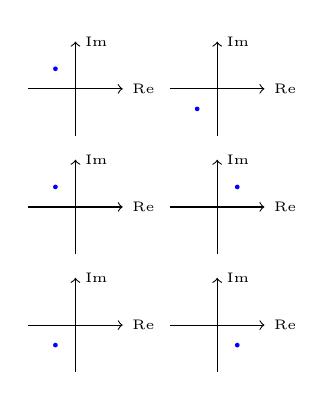
\begin{tikzpicture}[scale=0.6]
  \def\symbolsang{{-45, -135, 45, 135, 45, -45}}

  \foreach \y in {0, 1, 2} {
    \foreach \x in {0, 1} {
      \draw[black, ->] ({3 * \x - 1}, {2.5 * \y}) -- +(2, 0) node[right]{\tiny Re};
      \draw[black, ->] ({3 * \x}, {2.5 * \y - 1}) -- +(0, 2) node[right]{\tiny Im};

      \fill[blue]
      ({3 * \x - 0.6 * cos(\symbolsang[\y * 2 + \x])},  {2.5 * \y + 0.6 * sin(\symbolsang[\y * 2 + \x])}) circle(0.05);
    }
  }
\end{tikzpicture}
